\documentclass{cs-moi}
\usepackage{geometry}
\usepackage{graphicx}
\usepackage{hyperref}

\title{Projet Messagerie C}
\author{Wassim Ben Nacef - Nabil Bennacer - Max Chateau}
\date{Polytech Montpellier - IG 3} 

\begin{document}
\maketitle{}
\begin{center}
	
\includegraphics[width=0.3\linewidth]{logoPolytech.png}
\end{center}

\vspace{4pt}
    \hrule
\vspace{4pt}
  
\section{Introduction}
\textbf{BetterSkype} est un projet de messagerie en C fonctionnant avec un modele Client - Serveur via le terminal. Le code du projet est accessible sur Github :\\https://github.com/MaxbanCh/BetterSkype

\section{Developpement}
\subsection{Problematiques}
Les differentes problematiques a gerer seront les choix de protocoles reseaux, ainsi que le choix des processus ou des threads.

\subsection{Choix techniques}
En terme de communication nous avons fait le choix d'utiliser le protocole UDP pour les messages classiques, et TCP pour les envois de fichiers.

\begin{remarque}{Choix UDP + Processus}
     Ce choix s'explique d'une part pour des raisons de scalabilite et d'optimisation, dans la mesure ou ce protocole permet cote serveur de receptionner des messages independamment de la personne qui l'envoie, sans consacrer un thread pour chaque utilisateur, ce qui permet de ne pas consommer trop de ressources a grandes echelles, en plus de ne pas avoir a gerer pour $n$ utilisateurs, $n$ semaphores cote serveur.\\
     Afin de garantir l'integrite des messages, on va proceder a differentes verifications (nombres de paquets recus, nombre d'octets recu dans un paquet...) lors de l'envoi et de la reception des paquets, ce qui permet de garder l'efficacite de l'UDP dans la majorite des cas de succes.\\
     On aura donc cote serveur, un processus qui s'occupera de gerer la reception des messages utilisateurs, ainsi qu'un autre processus qui gerera le renvoi des messages aux utilisateurs concernes. Idem cote client pour la communication avec le serveur. Cela nous permettra d'utiliser la communication interprocessus avec les signaux.
\end{remarque} 

\subsection{Solutions mises en places}
\subsubsection{Gestion des messages}
On va utiliser une structure de message qui va contenir les differentes proprietes afin de garantir la bonne transmission ainsi que l'integrite des informations.\\
Lors de l'envoi on concatenera toutes les infos dans une chaine de caracteres, qui seront separees par des flags.

\begin{C}
    struct Message_S {
        char sender_ip[INET_ADDRSTRLEN];
        char dest_pseudo[PSEUDO_MAX];
        int  part_num;
        int  total_parts;
        char payload[BUFFER_MAX];
    };
    typedef struct Message_S Message;
\end{C}

\begin{figure}[h!]
    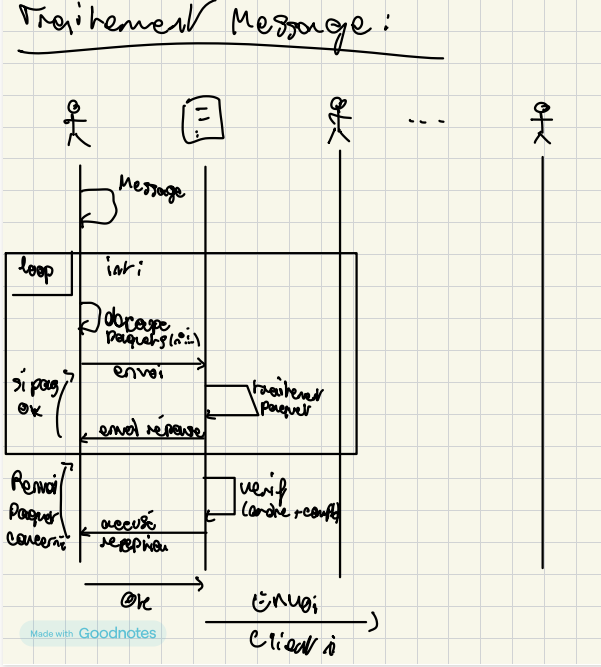
\includegraphics[width=0.7\linewidth]{diagMsg.png}
    \caption{Diagramme de sequence du fonctionnement des messages}
    \centering
\end{figure}


\subsubsection{Makefile}
Le projet sera fournit avec un makefile qui permettra de compiler automatiquement tout les fichiers necessaires au fonctionnement du projet, et de netoyer les fichiers auxiliares via une simple commande.\\

\subsubsection{}

\newpage
\section{Organisation}

\subsection{Diagramme de Gantt}

\begin{figure}[h!]
    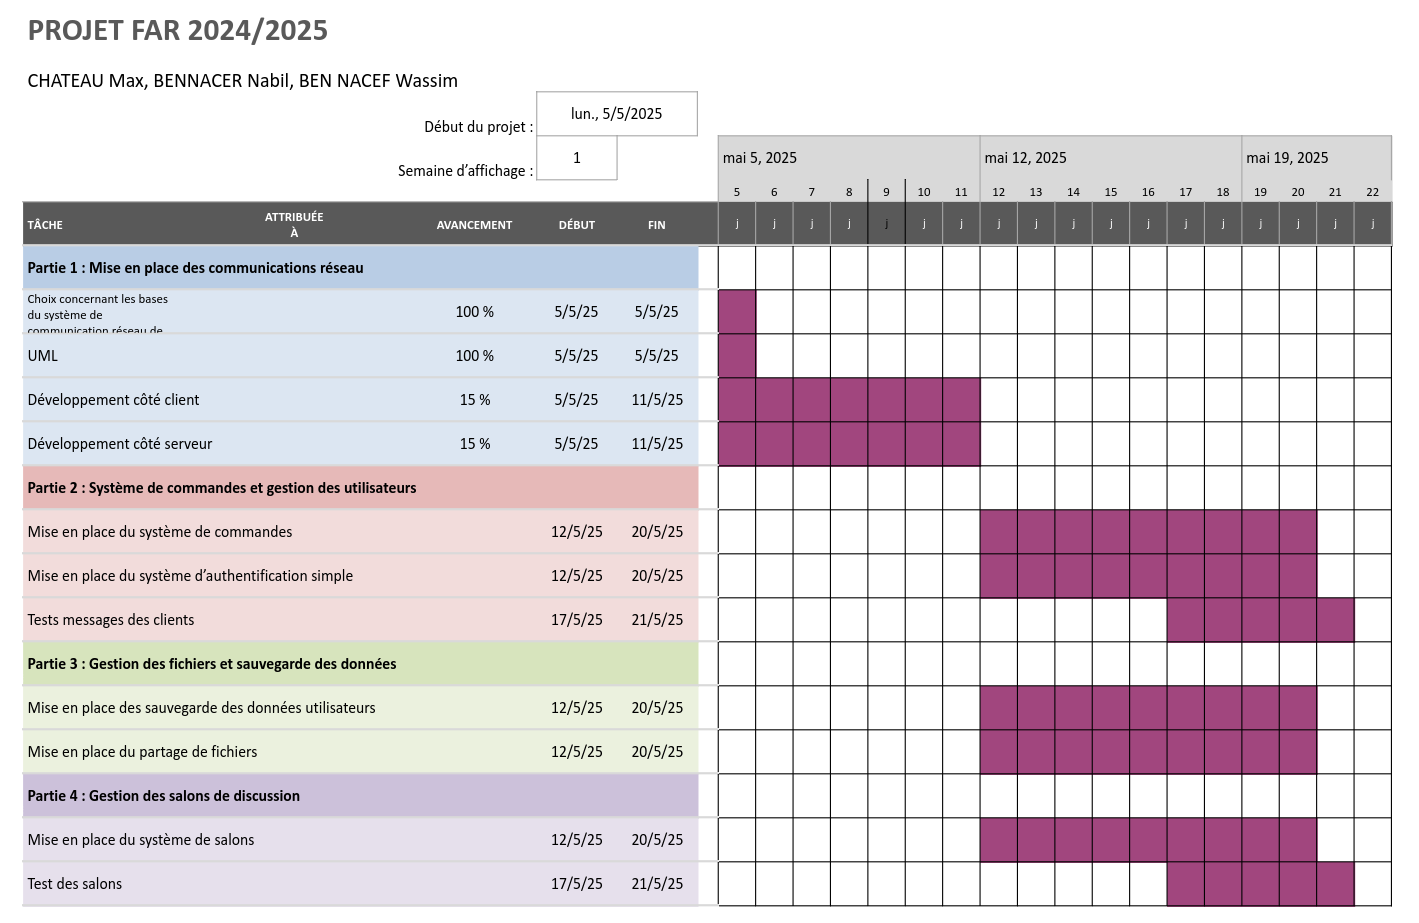
\includegraphics[width=0.95\linewidth]{Gantt.png}
    \caption{Diagramme de Gantt du projet}
    \centering
\end{figure}

\subsection{Detail}
Pour une breve explication de l'organisation, on a decide de se concentrer durant la premiere semaine sur la conception de la premiere partie afin d'etre sur de notre 

\section{Annexes}
Lien vers le Github du projet : https://github.com/MaxbanCh/BetterSkype
\end{document}